% Options for packages loaded elsewhere
\PassOptionsToPackage{unicode}{hyperref}
\PassOptionsToPackage{hyphens}{url}
%
\documentclass[
]{article}
\usepackage{amsmath,amssymb}
\usepackage{lmodern}
\usepackage{iftex}
\ifPDFTeX
  \usepackage[T1]{fontenc}
  \usepackage[utf8]{inputenc}
  \usepackage{textcomp} % provide euro and other symbols
\else % if luatex or xetex
  \usepackage{unicode-math}
  \defaultfontfeatures{Scale=MatchLowercase}
  \defaultfontfeatures[\rmfamily]{Ligatures=TeX,Scale=1}
\fi
% Use upquote if available, for straight quotes in verbatim environments
\IfFileExists{upquote.sty}{\usepackage{upquote}}{}
\IfFileExists{microtype.sty}{% use microtype if available
  \usepackage[]{microtype}
  \UseMicrotypeSet[protrusion]{basicmath} % disable protrusion for tt fonts
}{}
\makeatletter
\@ifundefined{KOMAClassName}{% if non-KOMA class
  \IfFileExists{parskip.sty}{%
    \usepackage{parskip}
  }{% else
    \setlength{\parindent}{0pt}
    \setlength{\parskip}{6pt plus 2pt minus 1pt}}
}{% if KOMA class
  \KOMAoptions{parskip=half}}
\makeatother
\usepackage{xcolor}
\IfFileExists{xurl.sty}{\usepackage{xurl}}{} % add URL line breaks if available
\IfFileExists{bookmark.sty}{\usepackage{bookmark}}{\usepackage{hyperref}}
\hypersetup{
  hidelinks,
  pdfcreator={LaTeX via pandoc}}
\urlstyle{same} % disable monospaced font for URLs
\usepackage{color}
\usepackage{fancyvrb}
\newcommand{\VerbBar}{|}
\newcommand{\VERB}{\Verb[commandchars=\\\{\}]}
\DefineVerbatimEnvironment{Highlighting}{Verbatim}{commandchars=\\\{\}}
% Add ',fontsize=\small' for more characters per line
\newenvironment{Shaded}{}{}
\newcommand{\AlertTok}[1]{\textcolor[rgb]{1.00,0.00,0.00}{\textbf{#1}}}
\newcommand{\AnnotationTok}[1]{\textcolor[rgb]{0.38,0.63,0.69}{\textbf{\textit{#1}}}}
\newcommand{\AttributeTok}[1]{\textcolor[rgb]{0.49,0.56,0.16}{#1}}
\newcommand{\BaseNTok}[1]{\textcolor[rgb]{0.25,0.63,0.44}{#1}}
\newcommand{\BuiltInTok}[1]{#1}
\newcommand{\CharTok}[1]{\textcolor[rgb]{0.25,0.44,0.63}{#1}}
\newcommand{\CommentTok}[1]{\textcolor[rgb]{0.38,0.63,0.69}{\textit{#1}}}
\newcommand{\CommentVarTok}[1]{\textcolor[rgb]{0.38,0.63,0.69}{\textbf{\textit{#1}}}}
\newcommand{\ConstantTok}[1]{\textcolor[rgb]{0.53,0.00,0.00}{#1}}
\newcommand{\ControlFlowTok}[1]{\textcolor[rgb]{0.00,0.44,0.13}{\textbf{#1}}}
\newcommand{\DataTypeTok}[1]{\textcolor[rgb]{0.56,0.13,0.00}{#1}}
\newcommand{\DecValTok}[1]{\textcolor[rgb]{0.25,0.63,0.44}{#1}}
\newcommand{\DocumentationTok}[1]{\textcolor[rgb]{0.73,0.13,0.13}{\textit{#1}}}
\newcommand{\ErrorTok}[1]{\textcolor[rgb]{1.00,0.00,0.00}{\textbf{#1}}}
\newcommand{\ExtensionTok}[1]{#1}
\newcommand{\FloatTok}[1]{\textcolor[rgb]{0.25,0.63,0.44}{#1}}
\newcommand{\FunctionTok}[1]{\textcolor[rgb]{0.02,0.16,0.49}{#1}}
\newcommand{\ImportTok}[1]{#1}
\newcommand{\InformationTok}[1]{\textcolor[rgb]{0.38,0.63,0.69}{\textbf{\textit{#1}}}}
\newcommand{\KeywordTok}[1]{\textcolor[rgb]{0.00,0.44,0.13}{\textbf{#1}}}
\newcommand{\NormalTok}[1]{#1}
\newcommand{\OperatorTok}[1]{\textcolor[rgb]{0.40,0.40,0.40}{#1}}
\newcommand{\OtherTok}[1]{\textcolor[rgb]{0.00,0.44,0.13}{#1}}
\newcommand{\PreprocessorTok}[1]{\textcolor[rgb]{0.74,0.48,0.00}{#1}}
\newcommand{\RegionMarkerTok}[1]{#1}
\newcommand{\SpecialCharTok}[1]{\textcolor[rgb]{0.25,0.44,0.63}{#1}}
\newcommand{\SpecialStringTok}[1]{\textcolor[rgb]{0.73,0.40,0.53}{#1}}
\newcommand{\StringTok}[1]{\textcolor[rgb]{0.25,0.44,0.63}{#1}}
\newcommand{\VariableTok}[1]{\textcolor[rgb]{0.10,0.09,0.49}{#1}}
\newcommand{\VerbatimStringTok}[1]{\textcolor[rgb]{0.25,0.44,0.63}{#1}}
\newcommand{\WarningTok}[1]{\textcolor[rgb]{0.38,0.63,0.69}{\textbf{\textit{#1}}}}
\usepackage{longtable,booktabs,array}
\usepackage{calc} % for calculating minipage widths
% Correct order of tables after \paragraph or \subparagraph
\usepackage{etoolbox}
\makeatletter
\patchcmd\longtable{\par}{\if@noskipsec\mbox{}\fi\par}{}{}
\makeatother
% Allow footnotes in longtable head/foot
\IfFileExists{footnotehyper.sty}{\usepackage{footnotehyper}}{\usepackage{footnote}}
\makesavenoteenv{longtable}
\usepackage{graphicx}
\makeatletter
\def\maxwidth{\ifdim\Gin@nat@width>\linewidth\linewidth\else\Gin@nat@width\fi}
\def\maxheight{\ifdim\Gin@nat@height>\textheight\textheight\else\Gin@nat@height\fi}
\makeatother
% Scale images if necessary, so that they will not overflow the page
% margins by default, and it is still possible to overwrite the defaults
% using explicit options in \includegraphics[width, height, ...]{}
\setkeys{Gin}{width=\maxwidth,height=\maxheight,keepaspectratio}
% Set default figure placement to htbp
\makeatletter
\def\fps@figure{htbp}
\makeatother
\setlength{\emergencystretch}{3em} % prevent overfull lines
\providecommand{\tightlist}{%
  \setlength{\itemsep}{0pt}\setlength{\parskip}{0pt}}
\setcounter{secnumdepth}{-\maxdimen} % remove section numbering
\ifLuaTeX
  \usepackage{selnolig}  % disable illegal ligatures
\fi

\author{}
\date{}

\begin{document}

\hypertarget{introducciuxf3n-a-cuda}{%
\subsection{Introducción a CUDA}\label{introducciuxf3n-a-cuda}}

\hypertarget{laboratorio-2-de-programaciuxf3n-paralela}{%
\paragraph{Laboratorio 2 de Programación
paralela}\label{laboratorio-2-de-programaciuxf3n-paralela}}

\begin{center}\rule{0.5\linewidth}{0.5pt}\end{center}

\hypertarget{introducciuxf3n-y-objetivos-de-la-pruxe1ctica-revisar}{%
\subparagraph{Introducción y objetivos de la práctica
(Revisar)}\label{introducciuxf3n-y-objetivos-de-la-pruxe1ctica-revisar}}

En este segundo laboratorio de la asignatura, utilizamos el mismo
algoritmo de conversión de un espacio de color a otro, aunque esta vez
existe un cambio de paradigma. Hasta el momento habiamos visto como
exprimir los recursos de la \emph{CPU} para aplicar paralelismo mediante
la librería de \emph{OpenMP}. En esta práctica, no tan solo usaremos la
\emph{CPU} sino que también aprenderemos el entorno de programación
\emph{CUDA} para aplicar el algoritmo mencionado mediante el uso de las
\emph{GPU} de \emph{nVidia}. Veremos también como podemos mejorar
progresivamente el rendimiento de la gráfica de un apartado a otro,
teniendo en cuenta distintos factores; como el uso de la memoria
compartida (\emph{shared memory}) o el uso de \emph{streams}.

De manera secundária, también nos familiarizaremos con el entorno basado
en celdas de \emph{google collab}, el cual nos facilita el uso de
\emph{CUDA} y la implementación del algoritmo, sin necesidad de disponer
de una \emph{GPU} directamente.

En este informe iremos comentando las soluciones propuestas para cada
apartado. El problema de la conversión de color se basa en una imagen
con resolución \emph{4K}, y en contraste con la anterior práctica (donde
el espacio "origen" era \emph{GRB}) se va de un espacio \emph{BRG} a
\emph{RGBA}.

A continuación, apuntamos el modelo de gráfica \emph{nVidia} (junto con
algunas de sus especifícaciones) con el que se han ejecutado todas las
secciones:

\begin{quote}
Device name: Tesla T4\\
Memory Clock Rate (KHz): 5001000\\
Memory Bus Width (bits): 256\\
Peak Memory Bandwidth (GB/s): 320.064000
\end{quote}

\begin{center}\rule{0.5\linewidth}{0.5pt}\end{center}

\hypertarget{secciuxf3n-1}{%
\subparagraph{Sección 1}\label{secciuxf3n-1}}

En primer lugar se pide completar algunos métodos ya declarados;
\texttt{allocGPUData}, \texttt{copyAndInitializeGPUData} y
\texttt{freeCUDAPointers}. Hace falta recordar que si estamos realizando
llamadas a la \emph{CUDA Runtime API}, en este caso para las funciones
de gestión de memoria, conviene "envolver" la llamada con
\texttt{CU\_CHECK}. Dichas funciones siempre devuelven un código de
error. De este modo, si no se devuelve \texttt{cudaSuccess}, podemos
conocer que tipo de error se ha producido.

\begin{itemize}
\item
  \texttt{allocGPUData} para reservar memoria en el
  dispositivo\footnote{Dispositivo es otra forma de referirnos a la
    tarjeta gráfica o \emph{GPU}.}. En nuestro caso conviene reservar
  los punteros para la imagen en ambas codificaciones.
\item
  \texttt{copyAndInitializeGPUData} copiará la información de la imagen
  en \emph{GBR} inicializada en el \emph{host}, enviándola al
  \emph{device}. Acto seguido inicializa a 0 los punteros para la imagen
  \emph{RGBA}.
\item
  \texttt{freeCUDAPointers} libera la memoria reservada en el
  dispositivo. Internamente se emplea el \texttt{cudaDeviceReset}, con
  lo que hacemos es destruir y liberar todos los recursos asociados con
  el dispositivo actual en el proceso actual.
\end{itemize}

Una vez comprobada la correcta implementación de dichos métodos, entre
otros, todos ellos incluidos en \texttt{experiment.h}, pasamos a la
implementación de la función de conversión; \texttt{convertBRG2RGBA}. En
\emph{OpenMP} paralelizamos los bucles \emph{for}, pero como ya he
mencionado en la introducción existe un cambio en la visión de como
programar en este entorno. Ahora lo que tenemos son los llamados
\emph{kernels}. Cada \emph{kernel} será ejecutado por los hilos de cada
\texttt{block}, de cada \texttt{grid} definidos antes del procesado.
Para esta sección implementamos un \emph{kernel} bidimensional, donde
emplearemos las coordenadas \emph{2D} de cada hilo para indexar cada
píxel en la imagen y realizar la conversión. Para seleccionar dichas
coordenadas, aprovechamos la fórmula vista en clase para identificar
unívocamente cada \emph{thread}:

\begin{Shaded}
\begin{Highlighting}[]
\DataTypeTok{int}\NormalTok{ x }\OperatorTok{=}\NormalTok{ threadIdx}\OperatorTok{.}\NormalTok{x }\OperatorTok{+} \OperatorTok{(}\NormalTok{blockIdx}\OperatorTok{.}\NormalTok{x }\OperatorTok{*}\NormalTok{ blockDim}\OperatorTok{.}\NormalTok{x}\OperatorTok{);} 
\DataTypeTok{int}\NormalTok{ y }\OperatorTok{=}\NormalTok{ threadIdx}\OperatorTok{.}\NormalTok{y }\OperatorTok{+} \OperatorTok{(}\NormalTok{blockIdx}\OperatorTok{.}\NormalTok{y }\OperatorTok{*}\NormalTok{ blockDim}\OperatorTok{.}\NormalTok{y}\OperatorTok{);} 
\end{Highlighting}
\end{Shaded}

De este modo pasamos de la posición relativa del hilo en cada
\texttt{block}, a la posición "general" dentro de cada \texttt{grid}.

Con esta implementación, para 100 iteraciones, obtenemos un tiempo de
ejecución de 48666us y \texttt{Executed!!\ Results\ OK.}.

\begin{center}\rule{0.5\linewidth}{0.5pt}\end{center}

\hypertarget{secciuxf3n-2}{%
\subparagraph{Sección 2}\label{secciuxf3n-2}}

En esta sección se pide adaptar de nuevo el código para una
\texttt{grid}unidimensional. Tal y como se puede ver en la función
\texttt{executeKernelconvertBRG2RGBA}, pasamos a tener un
\texttt{block}y una \texttt{grid} cuyas dimensiones vienen definidas por
la constante con valor 256 \texttt{BLOCK\_SIZE}. También se pide probar
con diferentes valores para esta constante.

En el \emph{kernel} \texttt{convertBRG2RGBA}, modificaremos el código
anterior tratando ambas imagenes como vectores unidimensionales.
Pasaremos de tener coordenadas \texttt{int\ x}, \texttt{int\ y}, a un
único valor \texttt{int\ x}. Por tanto únicamente emplearemos:

\begin{Shaded}
\begin{Highlighting}[]
\DataTypeTok{int}\NormalTok{ x }\OperatorTok{=}\NormalTok{ threadIdx}\OperatorTok{.}\NormalTok{x }\OperatorTok{+} \OperatorTok{(}\NormalTok{blockIdx}\OperatorTok{.}\NormalTok{x }\OperatorTok{*}\NormalTok{ blockDim}\OperatorTok{.}\NormalTok{x}\OperatorTok{);}
\end{Highlighting}
\end{Shaded}

Si comparamos los resultados con el apartado anterior, para un número
diferente de iteraciones (con un \texttt{BLOCK\_SIZE\ =\ 256}),
obtenemos los siguientes tiempos:

\begin{longtable}[]{@{}lll@{}}
\toprule
Iteraciones & Sección 1 (us) & Sección 2 (us) \\
\midrule
\endhead
100 & 48666 & 39876 \\
1000 & 420091 & 368419 \\
10000 & 3693547 & 3599177 \\
\bottomrule
\end{longtable}

Como se puede observar en los anteriores resultados, existe una mejora
significativa por lo que respecta al primer apartado. Hemos de revisar
un concepto que ya salió en el anterior apartado; localidad de datos.
Las lecturas entre posiciones de memoria consecutivas se dan más
fácilmente al tratar la imagen como array unidimensional, en contraste a
utilizar \emph{x} e \emph{y} para indexar cada píxel.

Por otro lado si variamos el tamaño de cada bloque o
\texttt{BLOCK\_SIZE}:

\begin{longtable}[]{@{}ll@{}}
\toprule
BLOCK\_SIZE & Sección 2 (us) \\
\midrule
\endhead
256 & 39876 \\
512 & 42209 \\
1024 (max) & 43650 \\
128 & 39378 \\
64 & 40031 \\
\bottomrule
\end{longtable}

Si tomamos como mejor en rendimiento, el modelo de la sección 2 y tan
solo variamos el tamaño del bloque, obtenemos el mejor tiempo en dividir
entre dos el valor inicial, es decir en \texttt{BLOCK\_SIZE\ =\ 128}.

\begin{center}\rule{0.5\linewidth}{0.5pt}\end{center}

\hypertarget{secciuxf3n-3}{%
\subparagraph{Sección 3}\label{secciuxf3n-3}}

Para este apartado continuaremos con el \texttt{BLOCK\_SIZE} que nos dió
mejores resultados en el anterior. Trataremos de optimizar los accesos a
memoria en contraste con las anteriores secciones, con la condición de
no emplear aún la \emph{memoria compartida}. La solución propuesta para
este apartado pasa por, inicialmente, calcular la coordenada del píxel
mediante la formula que hemos utilizado con anterioridad. En la sección
dos, estamos realizando "demasiados" accesos a la \emph{memoria global}
del dispositivo. En concreto para recuperar cada uno de los valores de
cada canal del píxel \emph{BRG}, para acabar asignandolos al nuevo píxel
en codificación \emph{RGBA} (añadiendo 255 para el factor de opacidad),
uno por uno. La solución que se propone es; traer de golpe el
\texttt{uchar3\ brg{[}x{]}} (donde \emph{x} es el indíce del píxel
dentro de la imagen) a una variable estática temporal \texttt{tmp}, con
lo que reducimos los accesos a \emph{memoria global}. Para asignar el
nuevo píxel convertido a \emph{RGBA}, tan solo debemos utilizar
\texttt{make\_uchar4} además del índice \emph{x}, accediendo a los
valores del temporal (a nivel de memoria reduce el coste de acceso al
estar en \emph{memoria privada}) uno a uno. Para ver mejor esta
conversión, se detallan las dos siguientes líneas:

\begin{Shaded}
\begin{Highlighting}[]
	\CommentTok{// Protection to avoid segmentation fault}
	\ControlFlowTok{if} \OperatorTok{(}\NormalTok{x }\OperatorTok{\textless{}}\NormalTok{ width }\OperatorTok{*}\NormalTok{ height}\OperatorTok{)} \OperatorTok{\{}
\NormalTok{      uchar3 tmp }\OperatorTok{=}\NormalTok{ brg}\OperatorTok{[}\NormalTok{x}\OperatorTok{];} \CommentTok{// we copy the whole uchar3 to private memory }
\NormalTok{      rgba}\OperatorTok{[}\NormalTok{x}\OperatorTok{]} \OperatorTok{=}\NormalTok{ make\_uchar4}\OperatorTok{(}\NormalTok{tmp}\OperatorTok{.}\NormalTok{y}\OperatorTok{,}\NormalTok{ tmp}\OperatorTok{.}\NormalTok{z}\OperatorTok{,}\NormalTok{ tmp}\OperatorTok{.}\NormalTok{x}\OperatorTok{,} \DecValTok{255}\OperatorTok{);} \CommentTok{// write all the values at the same time}
	\OperatorTok{\}}
\end{Highlighting}
\end{Shaded}

El tiempo de ejecución se reduce significativamente a un valor de
29125us.

Por otro lado, se comenta si existe algun problema con los accesos a
memoria. A parte de que, al principio, se realizan demasiados accesos,
si tomamos en cuenta que la memoria de la \emph{GPU} esta estructurada
en \emph{palabras} de \emph{4 bytes} en \emph{4 bytes}, existirá un
problema parecido al que ya vimos en el primer laboratorio con
\emph{OpenMP}. Anteriormente lo remediamos empleando el
\texttt{\_\_attribute\_\_((aligned(4)))}, de manera que, los píxeles que
ocupaban \emph{3 bytes} quedaban alineados y reduciamos los ciclos por
acceso a un número justo y necesario. En esta ocasión ocurre lo mismo.
Excepto el primer y último hilo, cada uno de ellos \emph{(t1, t2 ...
tn-2)}, realizará dos accesos por píxel dado que cada píxel en
\emph{BRG} ocupa \emph{3 bytes}, y como hemos dicho la estructura de la
memoria es de \emph{4 bytes} en \emph{4 bytes}. Pero esta vez el
compilador \emph{nvcc} no nos ayuda de la misma manera, con lo que no
obtenemos lecturas coalescentes. Este es el principal problema que se
solucionará con la implementación de las siguientes secciones.

\begin{center}\rule{0.5\linewidth}{0.5pt}\end{center}

\hypertarget{secciuxf3n-4}{%
\subparagraph{Sección 4}\label{secciuxf3n-4}}

La explicación de la solución a el problema anterior se hace explícita
en el \emph{pdf} del enunciado de la práctica. Como vemos en la
solución, se propone traer la información de la imagen \emph{BRG} (donde
cada píxel supone un espacio de \emph{3 bytes}) en grupos de \emph{4
bytes}. De esta manera podemos tener un único acceso por \emph{thread},
para leer la totalidad de los datos de la imagen en \emph{BRG}. Para
realizar este "truco", lo que haremos será calcular la posición de cada
hilo cuando leemos \emph{BRG} como si tuviera elementos de \emph{4
bytes}, mediante la constante \texttt{N\_ELEMS\_3\_4\_TBLOCK}. Con este
cálculo, únicamente utilizamos el 75\% de los hilos de cada bloque, con
lo cual, se requiere de un número mayor de bloques para traer toda la
imagen. Calcularemos el índice de cada lectura, por lo tanto, de la
siguiente forma:

\begin{Shaded}
\begin{Highlighting}[]
\DataTypeTok{int}\NormalTok{ position }\OperatorTok{=}\NormalTok{ threadIdx}\OperatorTok{.}\NormalTok{x }\OperatorTok{+} \OperatorTok{(}\NormalTok{blockIdx}\OperatorTok{.}\NormalTok{x }\OperatorTok{*}\NormalTok{ N\_ELEMS\_3\_4\_TBLOCK}\OperatorTok{);} \CommentTok{// use N\_ELEMS\_3\_4\_TBLOCK to compute the position of each thread when we read brg as if it had elements of 4 bytes}
\end{Highlighting}
\end{Shaded}

En esta sección, transferimos los datos desde \emph{device memory} a
\emph{shared memory}, una memoria de menos latencia y de menos tamaño,
pero que a la vez es compartida por todos los bloques de un
\emph{Streaming Multiprocessor}. Es decir, cada \emph{thread} de un
bloque particular posee una memoria compartida en común con los otros
\emph{threads} del mismo bloque. Debemos tener cuidado y saber buscar el
balance en la \emph{memoria compartida} usada para cada
\emph{threadblock}, ya que como he dicho esta memoria esta físicamente
compartida por los mismos. \\
Asignaremos cada \emph{palabra}, al array de \emph{memoria compartida}
con nombre \texttt{bgrShared}. Después de esta transferencia de datos de
\emph{memoria global} a \emph{compartida}, debemos explicitar una
barrera para sincronizar todos los hilos de ejecución, con tal de
asegurarnos que los datos son correctos antes de proceder. Una vez
sincronizamos, continuamos recalculando la posición de cada píxel para
asignar el nuevo bloque de \emph{RGBA}. Para ello, utilizamos de nuevo
la función \texttt{make\_uchar4}.

Como hemos podido ver, hemos solucionado el problema de la alineación de
memoria para la lectura coalescente de cada \emph{thread}. Por lo que
los accesos para traer cada píxel del vector \texttt{brg}, disminuyen a
1 por \emph{thread} en lugar de 2. \\
Por otro lado;

\begin{itemize}
\item
  utilizamos más accesos de memoria (en concreto dos accesos a
  \emph{memoria compartida} adicionales, aunque si es verdad que son más
  "baratos"),
\end{itemize}

\begin{itemize}
\item
  utilizamos la sincronización de hilos mediante el
  \texttt{syncthreads},
\item
  y usamos un mayor número de bloques (los cuales deben sincronizarse y
  a la vez compartir memoria).
\end{itemize}

Parece que la solución al anterior problema sale mas cara. Como
consecuencia, este nuevo \emph{kernel} disminuye el rendimiento en
contraste al apartado anterior, con un tiempo de 32300us. En el próximo
apartado, se implementa un algoritmo en el que, cada tres bloques de
\emph{4 bytes}, se genera la información necesaria para la conversión de
4 píxeles por un mismo \emph{thread}. Utilizaremos también \emph{memoria
compartida}.

\begin{center}\rule{0.5\linewidth}{0.5pt}\end{center}

\hypertarget{secciuxf3n-5}{%
\subparagraph{Sección 5}\label{secciuxf3n-5}}

Este ejercicio se basa en la implentación del algoritmo del enunciado de
la práctica. Se ha seguido al pie de la letra, la implementación
indicada en el \emph{pdf}. \\
Inicialmente procederemos de la misma forma que en la anterior sección
(para traer toda la imagen a \emph{shared memory}), hasta llegar a la
sincronización. A partir de este punto utilizaremos una cuarta parte del
total de hilos para escribir 128 píxeles en el conjunto \emph{RGBA}.
Para ello emplearemos \texttt{pix\_write} un vector de memoria
compartida que será el encargado de guardar los resultados de la
conversión. Cada hilo puede realizar la misma tarea, ya que en coger 3
\emph{palabras} de 4 \emph{bytes}, obtenemos 4 píxeles en total (de la
codificación \emph{BRG}). Con esto cada hilo puede escribir en
\texttt{rgba}, cuatro píxeles, con lo que finalmente conseguimos
escribir un total de 128 píxeles. El algorítmo, esta pensado para
solucionar el problema de los múltiples accesos a memoria que se da
anteriormente y se describe en las siguientes figuras:

(Procedimiento igual que en la sección 4):

\begin{figure}
\centering
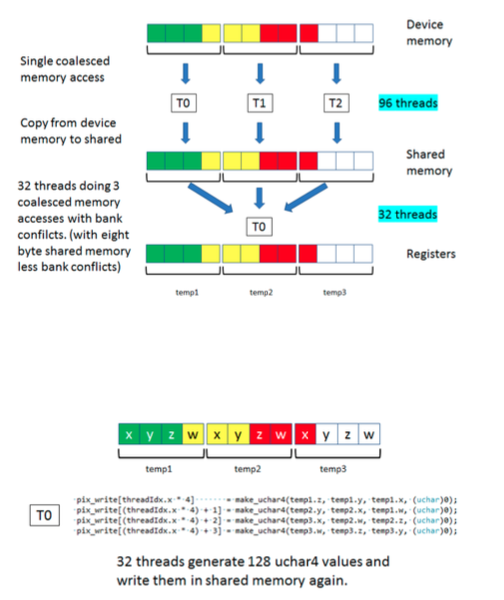
\includegraphics{/Users/marcosplazagonzalez/Desktop/Informe_Lab2CUDA_MarcosPlazaGonzalez/images/section5_1.png}
\caption{}
\end{figure}

(Procedimiento adicional con el que se realiza la conversión):

\begin{figure}
\centering
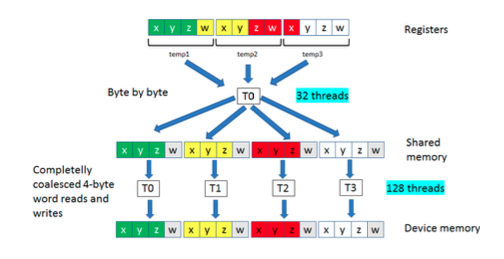
\includegraphics{/Users/marcosplazagonzalez/Desktop/Informe_Lab2CUDA_MarcosPlazaGonzalez/images/section5_2.png}
\caption{}
\end{figure}

De esta manera, estamos conservando siempre la coalescencia de las
lecturas y las escrituras. Cabe decir que para realizar la escritura de
\emph{memoria compartida} a \emph{memoria global}, escribiendo desde
\texttt{pix\_write} a el vector \texttt{rgba}, hace falta de nuevo,
sincronizar hilos y recalcular las posiciones de cada hilo que vaya a
realizar la transferencia. Con esto, junto a los accesos a memoria
añadidos en el ejercicio, el tiempo sube un poco más que en el anterior
apartado (36050us), aunque como siempre se obtiene
\texttt{Executed!!\ Results\ OK.}.

\begin{center}\rule{0.5\linewidth}{0.5pt}\end{center}

\hypertarget{secciuxf3n-6}{%
\subparagraph{Sección 6}\label{secciuxf3n-6}}

Por último, en este ejercicio se pide implementar el uso de
\emph{streams}, mediante un ejemplo dado. Cabe observar que el
\emph{kernel} será el mismo que en el ejercicio 3, que es el ejercicio
con el menor tiempo de ejecución en la conversión, pero como he dicho,
esta vez contaremos con \emph{streams}. \\
Dichos \emph{streams} sirven para que la ejecución de la \emph{CPU} al
mandar las instrucciones desde el \emph{host code} no se detenga y así
optimizar los tiempos. De este modo, además, se realizarán acciones
concurrentemente, si el \emph{stream} usado es diferente a 0
(\emph{stream} por defecto). Para ello debemos sobreescribir las
operaciones implementadas en el primer ejercicio; \texttt{allocGPUData},
\texttt{copyAndInitializeGPUData}, y \texttt{freeCUDAPointers}, mediante
el uso de operaciones no bloqueantes como:

\begin{itemize}
\item
  \texttt{cudaMemcpyAsync}
\item
  \texttt{cudaMemsetAsync}
\end{itemize}

Mediante las pertinentes modificaciones del código con el \emph{stream}
diferente a 0, para una sola iteración y para el mismo
\texttt{BLOCK\_SIZE\ =\ 128}, obtenemos un tiempo de conversión igual a
32352us. Por otro lado, el tiempo empleado por la \emph{CPU} para la
comunicación con la \emph{GPU} es de 58653us. \\
Si establecemos el \emph{stream} por defecto obtenemos los siguientes
tiempos;

\begin{center}\rule{0.5\linewidth}{0.5pt}\end{center}

\hypertarget{conclusiones}{%
\subparagraph{Conclusiones}\label{conclusiones}}

\begin{center}\rule{0.5\linewidth}{0.5pt}\end{center}

\hypertarget{links-de-referencia}{%
\subparagraph{Links de referencia}\label{links-de-referencia}}

\begin{itemize}
\item
  \href{https://developer.nvidia.com/blog/cuda-refresher-cuda-programming-model/}{Repaso
  CUDA}
\item
  \href{https://docs.nvidia.com/cuda/cuda-c-best-practices-guide/index.html}{Mejores
  prácticas}
\item
  \href{https://developer.nvidia.com/blog/gpu-pro-tip-cuda-7-streams-simplify-concurrency/}{Streams}
\end{itemize}

\end{document}
